\cleardoublepage
\mbox{}

\lstset{
language=Python,
basicstyle=\small\sffamily,
numbers=left,
numberstyle=\tiny,
frame=tb,
columns=fullflexible,
showstringspaces=false
}

\chapter{Tecnología OpenVINO}
\label{ch:chapter3}

OpenVINO es un conjunto de herramientas multi plataforma desarrolladas por Intel, que facilita la transición entre entre los entornos de entrenamiento y producción de nuestro modelo de aprendizaje profundo.
A pesar de estar desarrollada por una empresa comercial como Intel, peternece al conjunto de aplicaciones de código abierto, de modo que se puede visualizar su código fuente, repotar fallos e incluso realizar aportaciones.
Podemos visualizar el diseño y el código de la aplicación en su repositorio oficial de Github \footnote{https://github.com/openvinotoolkit/openvino}.
El cometido principal de esta aplicación es la optimización del tiempo de inferencia de un modelo de Deep Learning previamente entrenado.
Para ello, OpenVINO dispone de su propio formato de definición de modelos.
Estos archivos son los que procesa su propia red de inferencia multi plataforma, ya que se encuentra preparada para poder trabajar con los mismos de manera concurrente, aprovechando así toda la potencia de los procesadores o GPU actuales.
En la siguiente figura~\ref{fig:Arquitectura de optimización de modelos con OpenVINO} se puede observar el flujo de trabajo que se ha seguido en este trabajo, haciendo uso de la herramienta OpenVINO
En primer lugar, optimizaremos la topología de nuestro modelo a uno preparado para ser procesado por la red de inferencia de alto rendimiento de OpenVINO\@.
Finalmente, nuestra red de inferencia será la que realice el trabajo de clasificación en el entorno de producción de nuestra aplicació



\begin{figure}
    \centering
    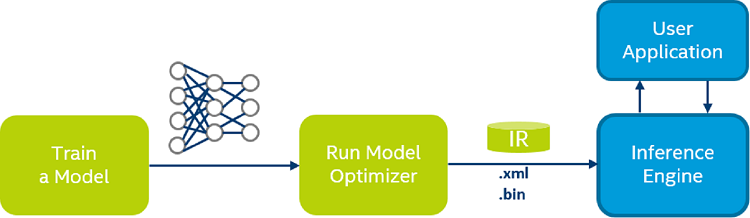
\includegraphics[width=0.8\textwidth]{images/chapter3/openvino_workflow.png}
    \caption{Arquitectura de optimización de modelos con OpenVINO}
    \label{fig:Arquitectura de optimización de modelos con OpenVINO}
\end{figure}


\section{Herramientas que lo componen}\label{sec:herramientas-que-lo-componen}
Esta tecnología desarrollada por intel tiene por objetivo principal la optimización de modelos de redes neuronales convolucionales para potenciar su velocidad de inferencia, mediante las distintas herramientas que lo componen.
OpenVINO es capaz de soportar distintos hardwares (FPGA, Intel movidius, procesamiento por GPU\@) y también varios sistemas operativos (Mac Os, Linux o Windows).
Las características principales de esta aplicación se resumen en dos puntos :
\begin{itemize}
    \item \textbf{Optimizador de modelos de deep learning}: Aplicación de interfaz de línea de comando, la cual usa como base modelos de frameworks populares como Caffe, TensorFlow, MXNet, Kaldi y ONNX para convertirlos a un modelo optimizado de OpenVINO.
    \item \textbf{Interfaz de inferencia de modelos de deep learning}: API de alto rendimiento multi plataforma para realizar la inferencia de manera rápida.
\end{itemize}

\subsection{Optimizador de modelos de deep learning}\label{subsec:optimizador-de-modelos-de-deep-learning}
Para poder realizar la optimización de nuestro modelo de deep learning previamente entrenado, se necesita el binario que contiene la topología de la red del modelo.
Una vez el optimizador de OpenVINO recibe como argumento nuestro modelo procede a realizar una conversión de cada capa interna de la red a una nueva capa.
Esta nueva capa, ya convertida al formato de OpenVINO, conserva los pesos de la red anterior,
sin embargo, está preparada para que la aplicación de inferencia de OpenVINO pueda leerla correctamente.
La herramienta de OpenVINO proporciona de manera genérica distintos scripts para realizar esta conversión.
Se incluyen diferentes ficheros de código fuente para los frameworks de Deep Learning más actuales, codificados en python y a los que se puede modifcar su código, aunque en principio no es necesario porque ya vienen preparados para funcionar.

\subsection{Interfaz de infernecia de modelos de deep learning}\label{subsec:interfaz-de-infernecia-de-modelos-de-deep-learning}
Con nuestro modelo y su topología convertida a un formato válido de OpenVINO, ya tenemos todo lo necesario para poder realizar clasificaciones con su interfaz de inferencia\@.
La optimización de inferencia se produce en este punto, donde cada capa de nuestro modelo original es procesada por la aplicación en un lenguaje de bajo nivel, optimizado para realizar operaciones vectoriales bajo total control del programador.
El lenguaje empleado para la codificación de la aplicación es C++ pese a que el programa pueda ser utilizado también en Python.
Esto se debe al uso de su API, que traduce las peticiones realizadas en Python al core de la interfaz, que es C++ puro.
Todas las capas usadas en este proyecto son compatibles de manera directa con las predefinidas por la interfaz de inferencia.
Entre otras cosas, OpenVINO nos da la posibilidad de añadir capas personalizadas, con el inconveniente de que deben ser programadas por el usuario de manera explícita en C++ para hacerlas compatibles con el resto de la aplicación.
Y, por supuesto, mantener estas nuevas capas a lo largo de las distintas actualizaciones y posibles cambios que pueda sufrir la aplicación.


\section{Conversión del modelo a la plataforma OpenVINO}\label{sec:conversión-del-modelo-a-la-plataforma-OpenVINO}
Para realizar la conversión del modelo, en primer lugar es necesaria la exportación del original de Tensorflow a un formato compatible con la red de optimización de modelos de OpenVINO.
La serialización por defecto de un modelo de Tensorflow puede incluir de manera independiente :

\begin{itemize}
    \item Un punto de control TensorFlow que contiene los pesos del modelo.
    \item Un prototipo 'SavedModel' que contiene el grafico subyacente de Tensorflow.
    Separa los graficos que se guardan para prediccion (servicio), capacitacion y evaluacion.
    Si el modelo no se compilo antes, solo el grafico de inferencia se exporta.
    \item La configuracion de arquitectura del modelo, si esta disponible
\end{itemize}

Los métodos exactos para la serializaciñon del modelo varían según la versión de Tensorflow, en cualquier caso la metodologíoa de conversión exacta utilizada
para este proyecto se puede encontrar en el repositorio de código fuente de este trabajo en Github : https://github.com/A-Ortiz-L/multispectral-imaging-cnn-final-degree-work
Este modelo de OpenVINO va a servir tanto de punto de partida para la optimización del mismo como para su uso directo en el servicio personalizado de Tensorflow para desplegar
modelos en producción.
Una vez exportado el modelo de deep learning al formato estándar de Tensorflow tendremos a nuestra disposición los ficheros necesarios para realizar la trasnformación de estos al formato de OpenVINO.
Para realizar esta operación se hace uso de la herramienta de Optimización de modelos, en concreto, con el script específico de Tensorflow, cuyo nombre
es \texttt{mo\_tf.py}

Este código fuente es ejecutado en la línea de comandos del sistema operativo correspondiente con los siguientes parámetros de entrada en la línea de comandos.


\begin{lstlisting}[caption=Comando de terminal para convertir un modelo Tensorflow a uno de OpenVINO.,
  label=a_label,
  float=t]
    mo_tf.py --input_model model.pb --input_model_is_text -b 1
\end{lstlisting}

En este comando epecifica con el flag \texttt{--input\_model\_is\_text} que nuestro fichero no está codificado en código binario, por lo que es texto plano.
Esta opción es totalmente configurable y depende del proceso de exportación.
Se ha encontrado útil la opción de exportaciòn a texto plano ya que de esta manera
se puede observar la arquitectura de la red y los pesos pertenecientes a cada capa.
Configuramos también el flag -b, esta opción determina el tamaño del batch que queremos especificar para la conversión, seleccionamos 1 porque en las entradas de nuestra red neuronal pueden propagarse valores
negativos, los cuales no son válidos para su procesamiento en OpenVINO.

\section{Inferencias.Tensorflow vs OpenVINO}\label{sec:inferencias.-Tensorflow-vs-OpenVINO}
Como se ha mencionado anteriormente Tensorflow posee su propio sistema de inferencia preparado para su uso productivo en un entorno real.
Esta sistema se llama Tensorflow serving, el cual incorpora un servidor codificado mediante el patrón diseño api rest, de modo que las peticiones
de inferencia se realizan al servidor por medio del protocolo de transmisión de datos http.
La aplicación de Tensorflow está diseñada para el escalado tanto en el número de modelos para los que puede recibir inferencias y sus versiones como para la escalabilidad en capacidad de cálculo.
El escalado de cáculo está preparado para funcionar en una arquitectura cluster, en este caso un cluster de contenedores como es kubernetes, por lo que el servidor puede ser
encapsulado en su totalidad en un contenedor de docker.
En este trabajo se ha trabajado con una versión encapsulada de docker, pero no con la extensibilidad del escalado con kubernetes.
La unidad de cálculo principal del sistema de inferncia también es configurable, perimitiendo así el uso tanto de cpu como de gpu.
Si se usa la opción de contenedores docker configurando una gpu es necesario configurar de manera esplícita este entorno.
En la siguiente figura podemos observar el diseño de la arquitectura de la aplicación~\ref{fig:Arquitectura de Tensorflow serving}
Una de las ventajas frente a usar el sistemá de inferencias clásico de Tensorflow es que la aplicación está preparada y optimizada para recibir tanto peticiones en streaming como en batch.
Adicionalmente reducimos el tamaño de las librerías a instalar al mínimo necesario para realizar las inferencias y configurar el servidor, por lo que la solución es más ligera y portable, evitando así
instalar todo el sistema de construcción de algoritmos y demás artefactos que incorpora la librerías de Tensorflow para construir redes neuronales.
La inicialización del servidor y los métodos necesarios para realizar la petición de inferencia se codifican de la siguiente manera :

\begin{lstlisting}[caption=Clase de Tensorflow de la aplicación del trabajo.,
  label=a_label,
  language=python]



class TensorflowNetwork:
    def __init__(self):
        self.model_uri = 'http://localhost:8501/v1/models/model:predict'
        self.init_tensorflow_serve()

    @staticmethod
    def shape_image(file_route):
        img_array = cv2.imread(file_route, cv2.IMREAD_GRAYSCALE)
        new_array = cv2.resize(img_array, (128, 128))
        img = new_array.reshape(-1, 128, 128, 1) / 255.0
        img = np.float32(img).tolist()
        return img

    def process_image(self, file_route) -> Tuple[bool, float]:
        start = time.time()
        image = self.shape_image(file_route)
        predict = self.network_request(image)
        return predict, (time.time() - start)

    def network_request(self, image) -> bool:
        headers = {"content-type": "application/json"}
        data = json.dumps({"signature_name": "serving_default", "instances": image})
        res = requests.post(self.model_uri, data=data,
                            headers=headers)
        predictions = json.loads(res.text)['predictions']
        predict = True if predictions[0][0] >= 0.5 else False
        return predict

    @staticmethod
    def init_tensorflow_serve():
        os.system('tensorflow_model_server '
                  '--rest_api_port=8501 --model_name=model '
                  '--model_base_path=/app/model &')
\end{lstlisting}
En la inicialización de la clase arrancamos el servidor rest, el cual funcionará de manera transparente para el usuario de nuestra aplicación, ya que el mismo se ejecuta en la red
local de nuestro servidor principal


\begin{figure}[h]
    \centering
    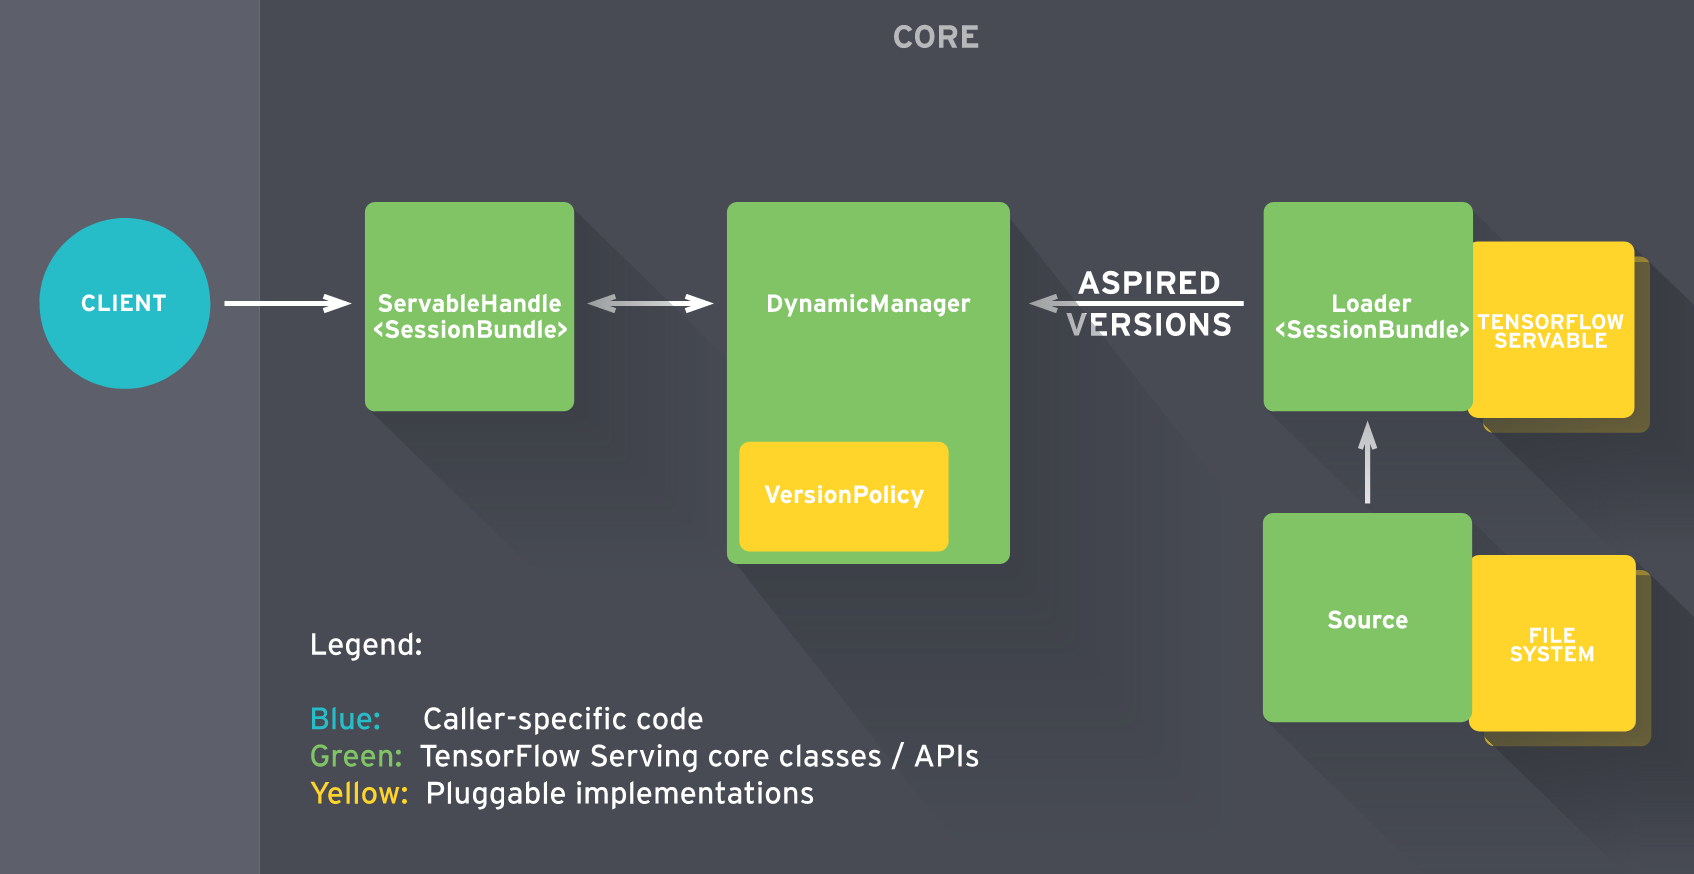
\includegraphics[width=0.8\textwidth]{images/chapter3/tf_serving_architecture.png}
    \caption{Arquitectura de Tensorflow serving}
    \label{fig:Arquitectura de Tensorflow serving}
\end{figure}

Por otro lado, OpenVINO también incorpora en su conjunto de herramientas un sistema de inferencia optimizado.
Al igual que el sistema de inferencia de Tensorflow, OpenVINO también puede configurar tanto cpu como gpu para realizar sus cálculos.
La aplicación de inferencia de OpenVINO usaada en este trabajo se codifica de manera íntegra haciendo uso del lenguaje de programación python,
por lo que el diseño software de este servicio y el procesamiento de las imágenes se codifica de la siguiente manera en el repositorio del trabajo.

\begin{lstlisting}[caption=Clase de OpenVINO de la aplicación del trabajo.,
  label=b_label,
  language=python]
    class OpenVinoNetwork:
    def __init__(self):
        self.plugin = IEPlugin(device='CPU')
        self.net = IENetwork(model=f'{pickle_dir}model.xml',
                             weights=f'{pickle_dir}model.bin')
        self.exec_net = self.plugin.load(network=self.net)

        self.input_blob = next(iter(self.net.inputs))
        self.out_blob = next(iter(self.net.outputs))
        self.net.batch_size = 1
        self.image_shape = 128

    def process_image(self, image_path) -> Tuple[bool, float]:
        start = time.time()
        image = self.shape_image(image_path)
        res = self.network_request(image)
        return res, time.time() - start

    def shape_image(self, file_route):
        image = cv2.imread(file_route, cv2.IMREAD_GRAYSCALE)
        image = cv2.resize(image, (self.image_shape, self.image_shape))
        image = image.reshape(self.image_shape, self.image_shape) / 255.0
        return image

    def network_request(self, image) -> bool:
        res = self.exec_net.infer(inputs={self.input_blob: image})
        res = res[self.out_blob]
        res = False if res < 0.5 else True
        return res
\end{lstlisting}

En la inicialización de la clase se lee el fichero ya optimizado del modelo de deep learning, también se inicia la clase
perteneciente a la api de inferencia de OpenVINO que se encarga de realizar las inferencia.
Se configuran métodos específicos para transformar la imagen a las dimensiones correspondientes y para hacer la petición a la red de inferencia.
La potencia de este modelo reside en la optimización que realiza la red en un lenguaje de bajo nivel, centrándose así en reducir los tiempos de inferencia.

En general, la aplicación de Tensorflow es más compleja a nivel de software, permitiendo su escalado en entornos de producción de manera muy simple.
Ambas soluciones implementan tecnologías de contenedores mantenidas de manera oficial por los fabricantes, por lo que el uso de Docker es la mejor opción para transportar
nuestras redes de inferencia a cuualquier sistema o dispositivo hardware.
En este punto, OpenVINO implementa de manera concreta soluciones para FPGA e intel movidius, por lo que las opciones de portabilidd son más amplias en esta tecnología.


